%
\section{Computer vision}
\label{sec:computer-vision}
Computer vision is a vast field, but can broadly be defined as the
transformation of data from a still image or video camera into
either a decision or a new representation to achieve some particular goal~\cite{kaehler2016learning}.

The input data may include some contextual information
such as `the camera is mounted in a car' or `laser range finder indicates an
object is 1 meter away.'
The decision might be `there is a person in this scene' or `there are 14
tumor cells on this slide.'
A new representation might mean turning a color image
into a grayscale image or removing camera motion from an image
sequence~\cite{kaehler2016learning}.

In this section, computer vision frameworks/libraries are listed, with special
focus on OpenCV, and computer vision algorithms for face detection and hand
gesture recognition are analyzed.
%
%
\subsection{Computer vision frameworks}
\label{sec:comp-visi-fram}
There are several noteworthy computer vision frameworks, namely~\cite{cv-frameworks-2020}:
\begin{enum-c}
\item \emph{Google Cloud's Vision API}:
it is an easy-to-use image recognition technology that
lets developers understand the content of an image by applying powerful machine
learning models. It enables key vision
detection features within an application ---  face, and landmark
detection, image labeling, \gls{ocr}, and explicit
content tagging --- and image classification into millions of predefined
categories.
\item \emph{YOLOv3}:
YOLO (You Only Look Once) is a state-of-the-art, real-time object detection
system among the most widely used deep learning-based object detection methods. It considers object detection as a regression problem,
directly predicting the class probabilities and bounding box offsets from full
images with a single feed-forward \gls{cnn}.
YOLOv3 eliminates region proposal generation and feature
resampling and encapsulates all stages in a single network to form a true
end-to-end detection system.
\item \emph{TensorFlow}:
it is a free, open-source framework for creating algorithms to develop a
user-friendly Graphical Framework called TensorFlow Graphical Framework
(TF-GraF) for object detection API, which is widely applied to solve complex
tasks efficiently in agriculture, engineering, and medicine.
The TF-GraF provides independent virtual environments for amateurs and beginners
to design, train, and deploy machine intelligence models without coding or
\gls{cli} in the client-side.
\item \emph{libfacedetection}:
it is an open-source library for face detection in images. It uses a pre-trained
\gls{cnn}, enabling face detection on inputs with a size greater than 10×10
pixels. The source code is not dependant on any other libraries. A C++ compiler
is required to compile the source under various platforms, such as Windows,
Linux, ARM, etc..
\item \emph{Raster Vision}:
it is an open-source Python framework to build computer vision models on
satellite, aerial, and other large sets of images (including oblique drone
imagery), using deep learning or machine learning models.
It has built-in support for chip classification, object detection, and semantic
segmentation with backbends using PyTorch and Tensorflow.
The framework is also extensible to new data sources, tasks (e.g., object
detection), backend (e.g., TF Object Detection API), and cloud providers.
\item \emph{SOD}:
it is an embedded, modern cross-platform computer vision and machine learning
software library.
It exposes a set of APIs for deep-learning, advanced media analysis, and
processing, including real-time, multi-class object detection, and model
training on embedded systems with limited computational resource and \gls{iot}
devices.
Designed for computational efficiency and with a strong focus on real-time
applications, SOD includes a comprehensive set of both classic and
state-of-the-art deep-neural networks with their pre-trained models.
Although it is open source, the pre-trained models are charged (one time fee
only -- up to 30 \gls{usd}).
\item \emph{Face\_recognition}:
  it is a facial recognition API for Python and the command line, built with
  deep learning using dlib60‘s state-of-the-art face recognition.
  The model has an accuracy of 99.38\% on the Labeled Faces in the Wild
  benchmark.
\item \emph{JeelizFaceFilter}:
it is a lightweight and robust face tracking library, designed for augmented reality face filters.
This JavaScript library can detect and track the face in real-time from the
webcam video feed captured, enabling the developers to solve computer-vision
problems directly from the browser.
The key features include face detection, face tracking, face rotation
detection, mouth opening detection, multiple face detection, and tracking, video
acquisition with \gls{hd} video ability, etc.
\item \emph{OpenCV}:
it is an open-source computer vision and machine learning software library,
built to provide a common infrastructure for computer vision applications and
accelerate the use of machine perception in commercial products.
OpenCV was designed for computational efficiency and with a strong focus on
real-time applications. It is written in optimized C++ and can take advantage of
multicore processors, with wrappers written in Python, Java, and Matlab, and
supporting Windows, Linux, Android and Mac OS.
The library has more than 2500 optimized algorithms, including a comprehensive
set of both classic and state-of-the-art computer vision and machine learning algorithms.
These algorithms can be used to detect and recognize faces, identify objects,
classify human actions in videos, track camera movements, track moving objects,
extract 3D models of objects and produce 3D point clouds from stereo cameras.
It can stitch images together to produce a high-resolution image of an entire
scene, find similar images from an image database, remove red eyes from images
taken using flash, follow eye movements, recognize scenery and establish markers to overlay it with augmented reality.
\end{enum-c}
%
%\subsubsection{OpenCV}
%\label{sec:opencv}
%
\subsection{Face detection}
\label{sec:face-detection}
Face detection has been studied for decades in the computer
vision literature. Modern face detection algorithms can be categorized into four categories~\cite{yang2016wider}:
cascade based methods, part based methods, channel feature based methods, and
neural network based methods. A detailed survey can be found in
~\cite{yang2002detecting, zhang2010survey}.

The seminal work by Viola and Jones~\cite{viola2004robust}
introduces integral image to compute Haar-like features in constant time.
These features are then used to learn AdaBoost classifier with cascade structure
for face detection.
Various later studies follow a similar pipeline, with SURF
cascade~\cite{li2013learning} achieving competitive performance.

Although the Viola-Jones are extremely fast, they require severe tunning to
prevent false-positives or complete misses.
In 2005, Dalal and Triggs~\cite{dalal2005histograms} demonstrated that the \gls{hog} image descriptor and
a Linear \gls{svm} could be used to train highly accurate object classifiers ---
or in their particular study, human detectors. However, due to the nature of
\gls{hog} that are only suited for frontal face detection as it is not invariant
to changes in rotation and viewing angle.

One of the well-known part based methods is \gls{dpm}~\cite{felzenszwalb2009object}. Deformable part
models define face as a collection of parts and model the connections
of parts through Latent \gls{svm}.
The part based methods are more robust to occlusion compared
with cascade-based methods.

\gls{acf} is first proposed by Dollar et al.~\cite{dollar2009pedestrian} to solve pedestrian detection.
Later on, Yang et al.~\cite{yang2014aggregate} applied this idea on face
detection. In particular, features such as gradient histogram, integral
histogram, and color channels are combined and used to learn boosting classifier
with cascade structure.

Recent studies~\cite{li2015convolutional, yang2015facial} show that face
detection can be further improved by using deep learning, leveraging the high
capacity of deep convolutional networks.

Considering a more pragmatic approach, the following tips are useful when
selecting a face detection method~\cite{pyimage-face-bestpractices}:
\begin{enum-c}
\item \emph{OpenCV's Haar cascades}:
      Use OpenCV's Haar cascades when speed is your primary concern (e.g., when
      considering an embedded device like the Raspberry Pi). Haar cascades
      aren't as accurate as their \gls{hog} + Linear \gls{svm} and deep learning-based
      counterparts, but they compensate it in raw speed. False-positive
      detections is highly likely and parameter tuning is required when calling
      \texttt{detectMultiScale}.
\item \emph{\gls{hog} + linear \gls{svm} detector}:
    Use \texttt{dlib's \gls{hog} + Linear \gls{svm}} detector when Haar cascades are not
    accurate enough, but you cannot commit to the computational requirements of
    a deep learning-based face detector.
    The \gls{hog} + Linear \gls{svm} object detector is a classic algorithm in the computer
    vision literature that is still relevant today.
    However, running \gls{hog} + Linear \gls{svm} on a \gls{cpu} will likely be too slow for an
    embedded device.
  \item \emph{CNN face detection}:
    Use dlib's \gls{cnn} face detection when requiring extremely accurate face
    detections.
   However, there is a tradeoff --- with
   higher accuracy comes slower run-time.
   This method cannot run in real-time on a laptop/desktop \gls{cpu}, and even with
   \gls{gpu} acceleration, you'll struggle to hit real-time performance.
  \item \emph{DNN face detector}:
    Use OpenCV's DNN face detector as a good balance. As a deep learning-based
    face detector, this method is accurate --- and since it's a shallow network
    with an single-shot detector backbone, it's easily capable of running in
    real-time on a \gls{cpu}. Furthermore, since you can use the model with
    OpenCV's \texttt{cv2.dnn} module, that also implies that (1) you can
    increase speed further by using a \gls{gpu} or (2) utilizing the Movidius
    NCS on your embedded device.
\end{enum-c}

% src: https://www.one-tab.com/page/1OS-OWq1RSKsGPIIvOj2JQ
%\subsubsection{Histogram of Oriented Gradients}
%\label{sec:hist-orient-grad}
%Deep learning methods for face detection can improve the face detection
%accuracy, but they require vast computational resources, making them unpractical
%for real-time detection. Viola-Jones detectors are extremely fast, but not
%reliable. As a trade-off between accuracy and speed, arises the \gls{hog}
%algorithm. Additionally, this algorithm comes built-in the major computer vision
%frameworks.

\subsubsection{Haar cascade classifier}
\label{sec:haar-casc-class}
Object detection using Haar feature-based cascade classifiers is an effective
method proposed by Viola and Jones~\cite{viola2001rapid}. It is a machine
learning based approach where a cascade function is trained from a lot of
positive and negative images. It is then used to detect objects in other images~\cite{opencv-haar-classif}.

The algorithm can be explained in four stages~\cite{haar-classif-explained}:
\begin{enum-c}
\item \emph{Calculating Haar Features}: the first step is to collect the Haar features. A Haar feature is essentially calculations that are performed on
adjacent rectangular regions at a specific location in a detection window. The
calculation involves summing the pixel intensities in each region and
calculating the differences between the sums. Some
examples of Haar features are illustrated in Fig.~\ref{fig:haar-features}.
\item \emph{Creating Integral Images}: instead of computing at every
pixel, sub-rectangles and its array references are created, which are then used
to compute the Haar features (see Fig.~\ref{fig:haar-integral}).
\item \emph{Using Adaboost}: to determine the best features from the hundreds of
  thousands of Haar features, one requires a machine learning model.
  Adaboost essentially chooses the best features and trains the classifiers to
  use them. It uses a combination of `weak classifiers' to create a `strong classifier' that the algorithm can use to detect objects.
Weak learners are created by moving a window over the input image, and computing Haar features for each
subsection of the image. This difference is compared to a learned threshold that
separates non-objects from objects. Because these are `weak classifiers', a large number of Haar features is needed for accuracy to form
a strong classifier (see Fig.~\ref{fig:boosting}). 
\item \emph{Implementing Cascading Classifiers}:
The cascade classifier is made up of a series of stages, where each stage is a
collection of weak learners (see Fig.~\ref{fig:cascade-implem}).
Weak learners are trained using boosting, which allows for a highly accurate
classifier from the mean prediction of all weak learners.

Based on this prediction, the classifier either decides to indicate an object
was found (positive) or move on to the next region (negative). Stages are designed to reject negative samples as fast as possible, because a
majority of the windows do not contain anything of interest.

It's important to maximize a low false negative rate, because classifying an object as a non-object will
severely impair your object detection algorithm, so it is critical to tune hyperparameters accordingly when training your model.
\end{enum-c}
%
\begin{figure}[htb!]
\centering
    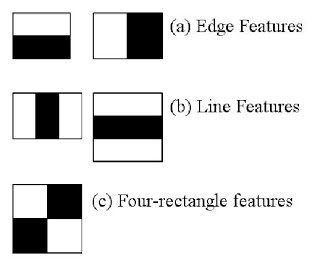
\includegraphics[width=0.4\columnwidth]{./img/haar-features.jpg}
  \caption{Examples of Haar features (withdrawn from~\cite{opencv-haar-classif})}%
\label{fig:haar-features}
\end{figure}
%
\begin{figure}[htb!]
\centering
    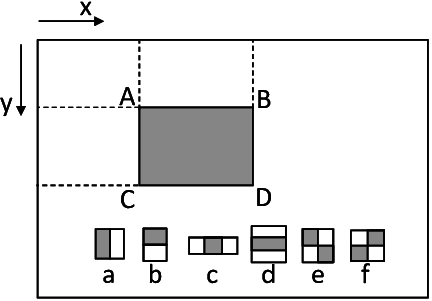
\includegraphics[width=0.4\columnwidth]{./img/haar-integral.png}
  \caption{Integral image creation illustration (withdrawn from~\cite{haar-classif-explained})}%
\label{fig:haar-integral}
\end{figure}
%
\begin{figure}[htb!]
\centering
    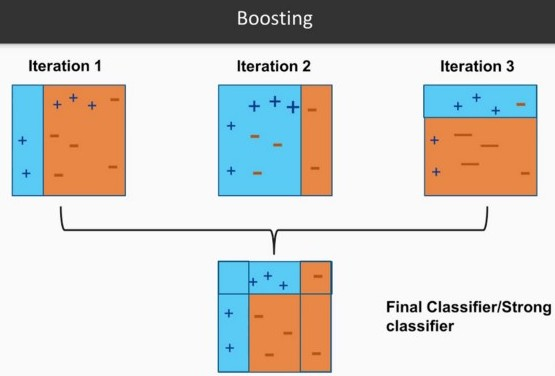
\includegraphics[width=0.6\columnwidth]{./img/boosting.jpeg}
  \caption{Illustration of a boosting algorithm (withdrawn from~\cite{haar-classif-explained})}%
\label{fig:boosting}
\end{figure}
%
\begin{figure}[htb!]
\centering
    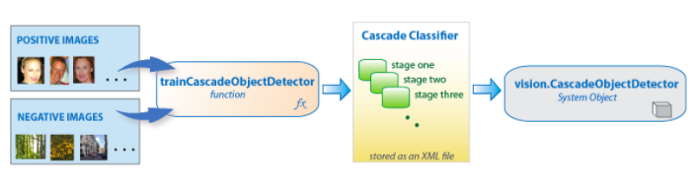
\includegraphics[width=1.0\columnwidth]{./img/cascade-implem.png}
  \caption{Flowchart of a cascade classifiers (withdrawn from~\cite{haar-classif-explained})}%
\label{fig:cascade-implem}
\end{figure}
%
\subsection{Hand gesture recognition}
\label{sec:hand-gest-recogn}
Human communication naturally relies on hand gestures for clarification of
intentions, thus making a viable bridge for interchanging information between
humans and computers~\cite{aashni2017international}.
The most notable applications of hand gesture recognition are: sign language
comprehension, robotics control, assisting disabled people, creation of
contactless user interfaces, game industry (e.g. Kinect), home automation,
clinical and health, virtual environments,
etc.~\cite{yasen2019systematic}.

However, the computational performance of recognizing hand gestures is affected
by the environmental surroundings (such as light, background, distance, skin
color) and the position and direction of
hand~\cite{vaibhavi2014review}. Additionally, hand gestures applications require
users to be well trained at employing and understanding the meaning of different
gestures, as for each application, a different group of gestures is used to
perform its operations~\cite{yasen2019systematic}.

In this section the hand gesture recognition process is explored, concerning
its workflow and most relevant methods.

The basic hand gesture recognition procedure is illustrated in Fig.~\ref{fig:hand-gesture-recog-procedure}, comprising
the following stages~\cite{yasen2019systematic}:
\begin{item-c}
\item \emph{image frame acquisition}:
  capture the human gesture image by
  computer, usually performed using a web camera or depth
  camera~\cite{choudhury2015review}.
  Special tools
  can be used such as wired or wireless gloves to detect hand movements, and
  motion sensing input devices (e.g., Kinect, Leap Motion, etc.) to capture the
  hand gestures and motions.
\item \emph{Hand tracking}:
  is the ability of the computer to trace the user
  hand and separate it from the background and from the surroundings
  objects~\cite{choudhury2015review}. This can be done using multi-scale color
  feature hierarchies that gives the users hand and the background different
  shades of colors to be able to identify and remove the background ---
  background subtraction and thresholding, or by using clustering algorithms
  that are capable of treating each finger as a cluster and removing the empty
  spaces in-between them~\cite{yasen2019systematic}.
\item \emph{Feature extraction}:
  The features vary depending on the application, with the most common being:
  fingers status, thumb status, skin color, alignments of fingers, and the palm
  position~\cite{choudhury2015review}. Several feature extraction methods can be
  used, such as Fourier descriptor method for capturing the palm, the fingers
  and the finger tips, or the centroid method which captures the essential
  structure of the hand~\cite{yasen2019systematic}.
\item \emph{Classification}: The features extracted are then sent to training
  and testing the classification algorithm
  (such as \gls{ann}, \gls{knn}, \gls{nb}, \gls{svm}, etc.)
  to reach the output gesture. A simple
  case of an output gesture can contain two classes to detect only two gestures
  such as open and closed hand gestures~\cite{yasen2019systematic}.
\end{item-c}
% HG procedure
\begin{figure}[!hbt]
\centering
    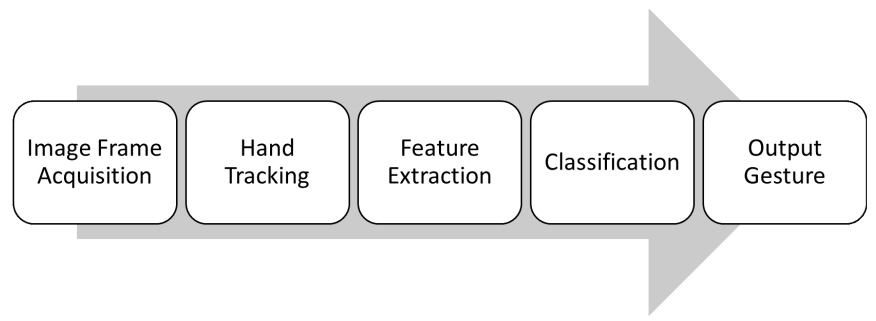
\includegraphics[width=0.6\textwidth]{./img/hand-gesture-recog-procedure.png}
  \caption{Basic steps of hand gesture recognition (withdrawn from~\cite{yasen2019systematic})}%
\label{fig:hand-gesture-recog-procedure}
\end{figure}

Fig.~\ref{fig:hand-gesture-procedure-simplified} illustrates an hand gesture
recognition workflow, materializing the aforementioned procedure, namely:
building a gesture dataset, tracking the hand and extracting the gesture by
creating a \gls{roi} and applying background subtraction and binary
thresholding, training the model with the new dataset, and perform the hand
gesture recognition using the predictive model.
%
\begin{figure}[!hbt]
\centering
    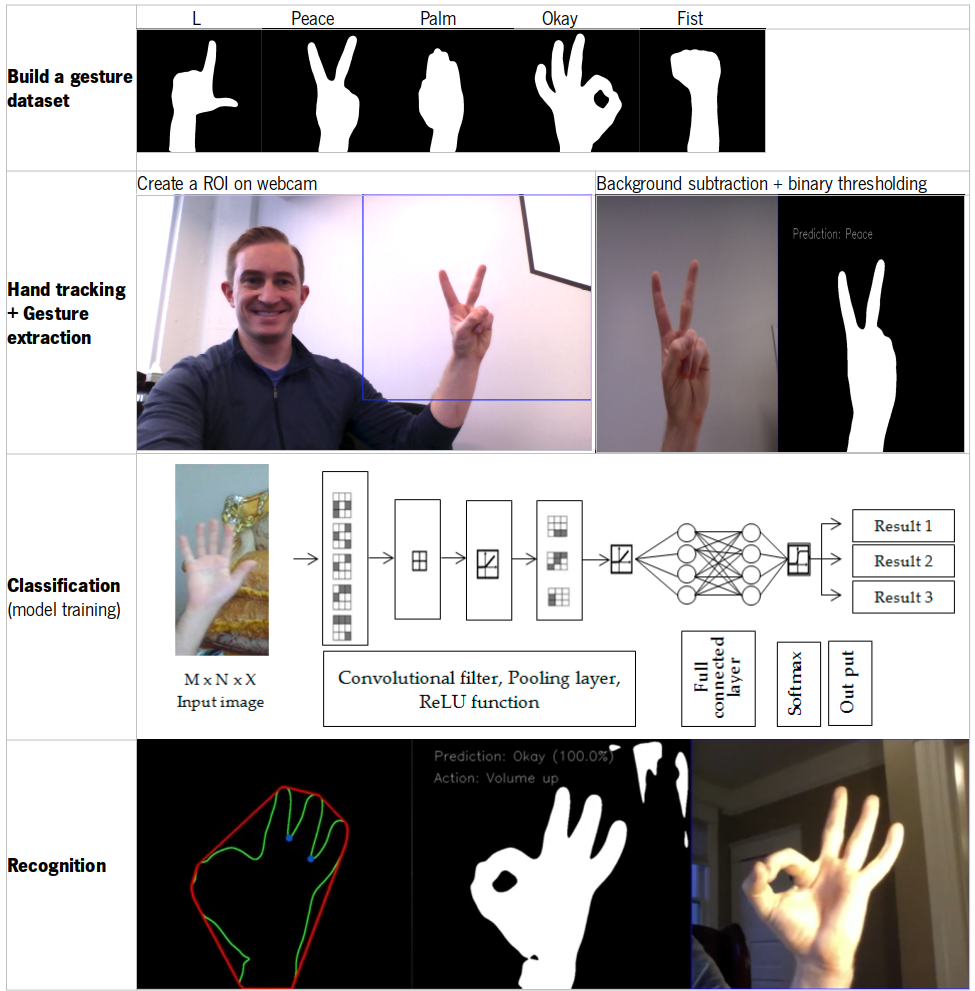
\includegraphics[width=1.0\textwidth]{./img/hand-gesture-procedure-simplified.png}
  \caption{Hand gesture recognition workflow illustrated: example --- adapted from~\cite{trainingNN4GestureDetection}~and~\cite{oudah2020hand}}%
\label{fig:hand-gesture-procedure-simplified}
\end{figure}


%\subsubsection{\emph{Hand gesture recognition techniques}}
%\label{sec:hand-gest-recogn-1}
%
%\paragraph{\textbf{Gesture acquisition methods}}
%
%\paragraph{\textbf{Feature extraction}}
%
%\paragraph{\textbf{Classification of hand gestures}}



%%% Local Variables:
%%% mode: latex
%%% TeX-master: "../../../dissertation"
%%% End:
